\section{Erstellung eines Modells zur Bodenatmung}
\label{sec-model}

Der Datensatz enthält sehr viele Features im Vergleich zur Anzahl an Messungen.
Der Suchraum der Variablenselektion wäre viel zu groß und muss demnach verkleinert werden.
Außerdem ist eine Schätzung von so vielen Parametern mit vergleichsweise wenigen Messungen auch statistisch zu ungenau.

\subsection{Test auf Vorliegen einer Normalverteilung}

Es werden nur normalverteilte (\it{Shapiro-Wilk}) und stark korrelierende (\it{Pearson}) Variablen in Betracht gezogen. Um \it{Pearson} als Korrelationskoeffizienten nutzen zu können, müssen die Messungen der Variablen normalverteilt sein. Um dies zu testen nutzen wir den \it{Shapiro-Wilk-Test}. Wenn der \it{p-Value} des \it{Shapiro-Wilk-Tests} größer als das Signifikanzniveau $\alpha=0.05$ ist, dann ist die Variable normalverteilt. Wie in Abbildung \ref{fig:shapiro} zu sehen ist, sind nur 14 der insgesamt 33 Variablen normalverteilt.

\begin{figure}[ht]
	\centering
	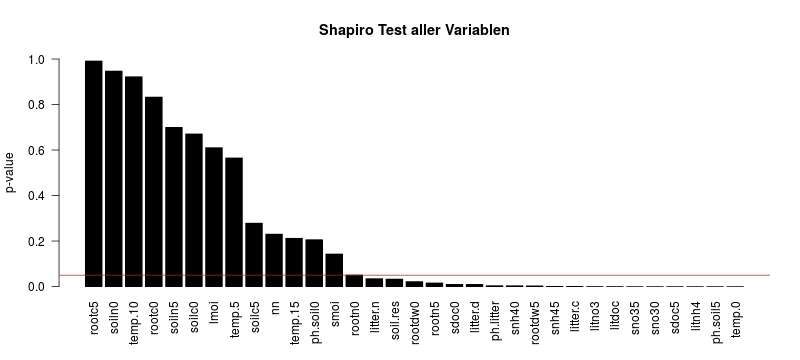
\includegraphics[width=\textwidth]{fig/model/normalverteilung-shapiro.png}
	\caption{\bf{P-Value des Shapiro-Wilk-Tests aller Variablen.}}
	\label{fig:shapiro}
\end{figure}

\subsection{Korrelationsanalyse}

Aus den normalverteilten Variablen werden die am stärksten korrelierenden Variablen ausgewählt (siehe Abbildung \ref{fig:pearson}). 

\begin{figure}
	\centering
	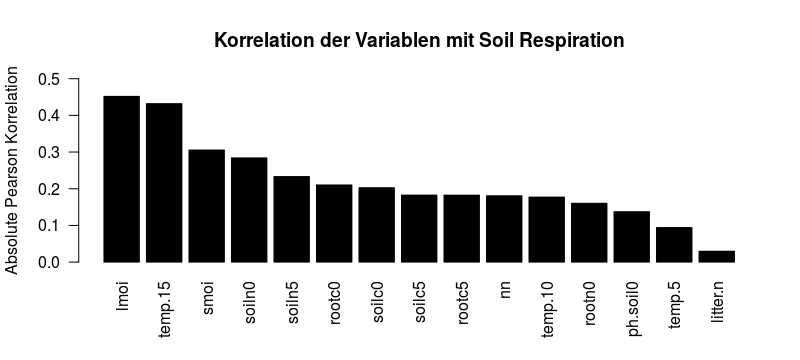
\includegraphics[width=\textwidth]{fig/model/correlation-pearson-normal.png}
	\caption{\bf{Pearson-Korrelation} der normalverteilten Einflussgrößen (\it{p-Value} $> 0.32$) mit der Bodenatmung.}
    \label{fig:pearson}
\end{figure}

\begin{itemize}
\item
  \emph{lmoi} relative Feuchte der Streuschicht (litter moisture)
\item
  \emph{temp15} Bodentemperatur in 15 cm Tiefe
\item
  \emph{smoi} relative Bodenfeuchte (soil moisture)
\end{itemize}

\subsection{Transformationen}

Lineare Modelle erfordern lineare Korrelationen.
Bei nicht linearen Korrelationen kann eine Linkfunktion als Transformation der Zufallsgröße verwendet werden, um die gewählte Messgröße zu linearisieren.
Soe \it{et. al.} verwendeten eine derartige Transformation vor allem für die Temperatur, da die Reaktionsgeschwindigkeit einer Reaktion exponentiell und nicht linear in Abhänigkeit der Temperatur verläuft.
Unsere Datenlage allerdings konnte die Notwendigkeit einer solchen Transformation nicht bestätigen (Vgl. Abbildung \ref{fig:temp}).
Eine hohe \it{Pearson}-Korelation bestätigte den Verdacht.
\begin{figure}
	\centering
	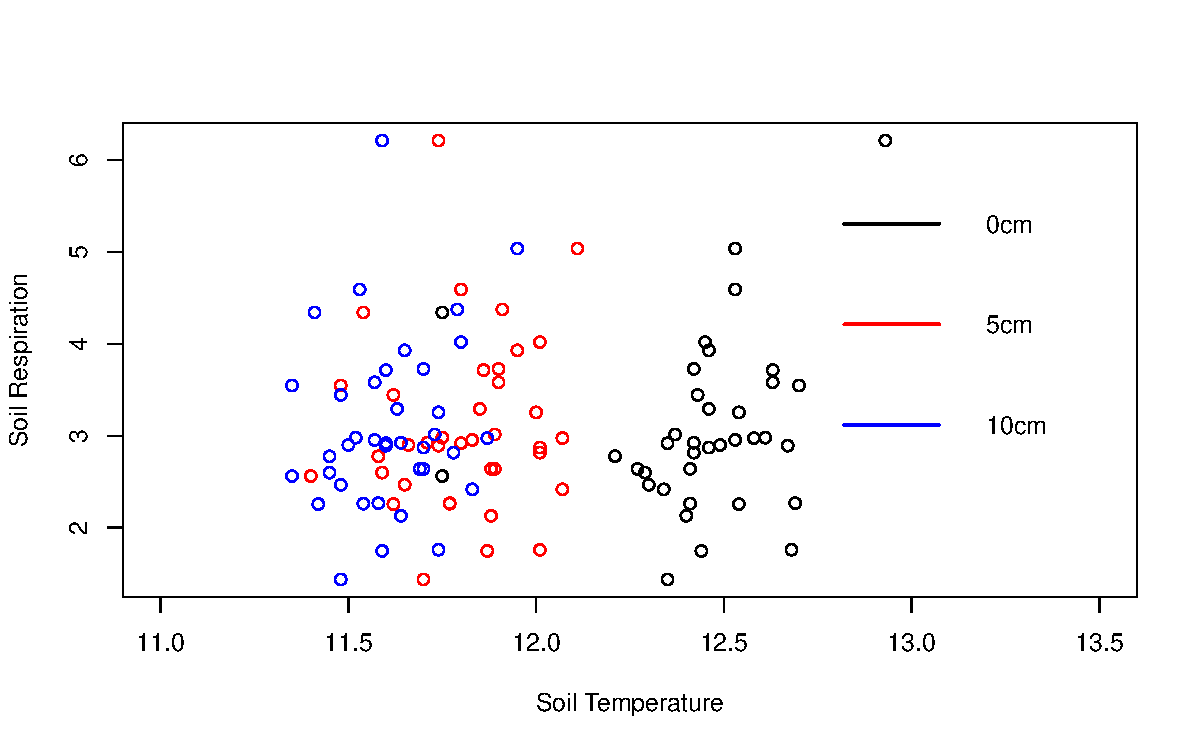
\includegraphics[width=\textwidth]{fig/model/temp-vs-resp.pdf}
	\caption{\bf{Bodenatmung in Abhänigkeit von der Temperatur.}
		 Es ist keine nichtlineare Korrelation der beiden Größen ersichtlich. }
	\label{fig:temp}
\end{figure}
Transformationen bringen keine deutlichen Verbesserungen der Variablen. 
Für diese Analyse wurde außerdem ein Scatterplot genutzt (Abbildung im Anhang).


\subsection{Variablenselektion}

Mit Hilfe des R-Pakets \emph{leaps} wird das Modell mit dem geringsten Wert des \emph{Bayesschem Informationskriteriums (BIC)} ausgewählt, welches das Kriterium der Modellqualität erfüllt.
In Abbildung \ref{fig:bic} sieht man, dass ein Hinzufügen der Variable $soiln0$ den BIC-Wert nur erhöhen würde.

\begin{figure}[ht]
	\centering
	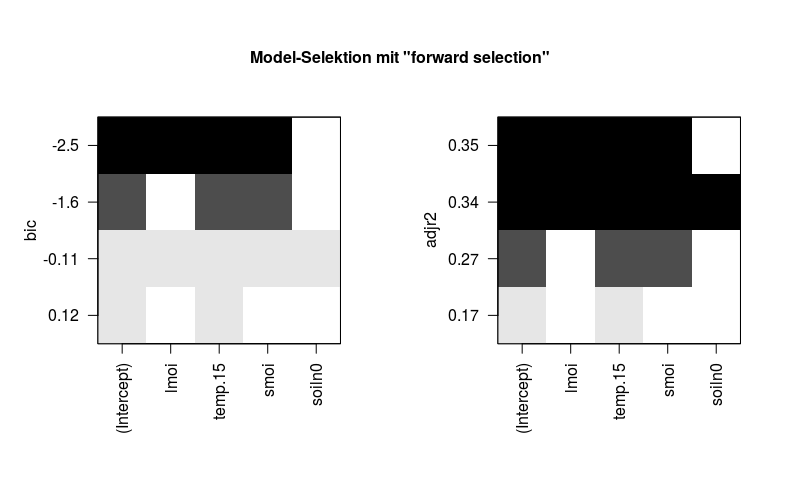
\includegraphics[width=\textwidth]{fig/model/variablenselektion-bic-adjr2.png}
	\caption{\bf{Variablenselektion mittels Bayesschem Informationskriterium (bic) und korrigiertes Bestimmtheitsmaß $\bar{R^2}$ (adjr22)}. Im linken Bild sieht man die Variablenselektion anhand des \emph{Bayesschem Informationskriteriums} und des \emph{korrigierte Bestimmtheitsmaßes}, die beide das Modell mit den ersten drei Variablen (\emph{lmoi, temp.15, smoi}) bevorzugt.}
    \label{fig:bic}
\end{figure}

\subsection{Ergebnis}
Bezüglich der Voraussetzungen der Normalverteilung, der Korrelation und des BICs wurde folgendes Modell zur Beschreibung der Bodenatmung ausgewählt:
$$soil.res = \vec{\beta} * (1,lmoi,temp15,smoi)^\text{T}$$

\subsection{Umsetzung mit R}

\begin{lstlisting}
# Test auf Normalverteilung
hainich.shapiro <- mapply(function(x) shapiro.test(x)$p.value,hainich)
hainich.normal <- hainich[names(hainich.shapiro[hainich.shapiro > 0.032])]
# Korrelation mit Pearson
hainich.pear <- abs(cor(hainich.normal))["soil.res",-16]
\end{lstlisting}
